\documentclass[11pt]{article}
\usepackage{fontspec}
\usepackage[utf8]{inputenc}
\setmainfont{Bodoni 72 Book}
\usepackage[paperwidth=11in,paperheight=8.5in,margin=1in,headheight=0.0in,footskip=0.5in,includehead,includefoot,portrait]{geometry}
\usepackage[absolute]{textpos}
\TPGrid[0.5in, 0.25in]{23}{24}
\parindent=0pt
\parskip=12pt
\usepackage{nopageno}
\usepackage{graphicx}
\graphicspath{ {./images/} }
\usepackage{amsmath}
\usepackage{tikz}
\newcommand*\circled[1]{\tikz[baseline=(char.base)]{
            \node[shape=circle,draw,inner sep=1pt] (char) {#1};}}

\begin{document}

\begin{center}
\huge FOREWORD
\end{center}

\begingroup
\begin{center}
\leftskip0.5in
More often called Sankt Walpurgisnacht, \textit{Hexennacht} traditionally commemorates the canonization of Saint Walpurga, the patroness of Eichstätt and Weilburg, Germany; Oudenarde, Veurne, and Antwerp, Belgium; and Tiel, Groningen, Arnhem, and Zutpenthe, Netherlands. She is revered for her battles against pests, disease, and witchcraft. The most contemporary observance of this festival is by The Satanic Temple as ``a solemn holiday to honor those who were victimized by superstition.''
\rightskip\leftskip
\phantom{text} \hfill -Trinton
\end{center}
\endgroup

\begingroup
\begin{center}
\rule{\textwidth}{1.6pt}\vspace*{-\baselineskip}\vspace*{1pt}
\rule{\textwidth}{0.4pt}\\[\baselineskip]
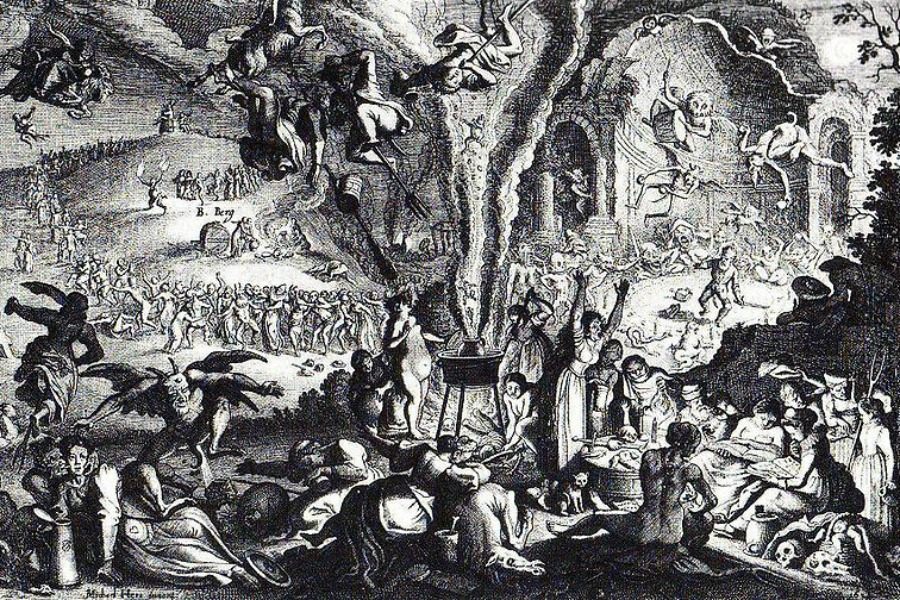
\includegraphics[scale=0.2]{hex_1.jpeg}
\rule{\textwidth}{0.4pt}\vspace*{-\baselineskip}\vspace{2pt}
\rule{\textwidth}{1.6pt}\\[\baselineskip]
\end{center}
\endgroup

\begingroup
\begin{center}
``There was weeping. \\ Weeping not for help or for comfort \\  A weapon, distant \\  Or disembodied \\ Not here, can't be with me \\ Can't. \\ I've only heard it once or twice, \\ Or perhaps a thousand times. \\ I can't be sure.''  -Trinton
\end{center}
\endgroup
\end{document}